We target a specific but very common use case (Figure~\ref{fig:usecase}). A researcher has written a paper with empirical content, and is required by the journal's data and code availability policy to prepare a ``replication package.'' The journal's policy requires that the code and data be accessible to others, but does not require deposit of the materials as a ``supplementary file,'' i.e., as a ZIP file on their website.\footnote{In fact, some journals may not offer that option.} However, in all cases, the journal wishes to ascertain three key attributes of the replication package or packages:
\begin{itemize}
    \item the \textit{existence} of the package
    \item the \textit{access rules} to the package (license, terms of use)
    \item the \textit{persistence} of the package
\end{itemize}
In an ideal scenario, the existence of the package can be easily ascertained in a reputable repository, it is made available under an well-specified (ideally open) license, and it is available ``forever''. When the journal manages its own repository, these attributes are known. When the package is available elsewhere, these attributes need to be discovered. Furthermore,  this needs to happen in a scalable,  automated, and reusable fashion, as it should be feasible to do so for all articles, submitted to any journal. However, in our use cases, the data used by the author is in fact re-used, secondary-use data, where the source data may not be in a traditional trusted repository. This, after all, is the whole point of FAIR: to be able to re-use existing data. And yet, the availability of metadata in such cases is problematic. 

\begin{figure}
    \centering
    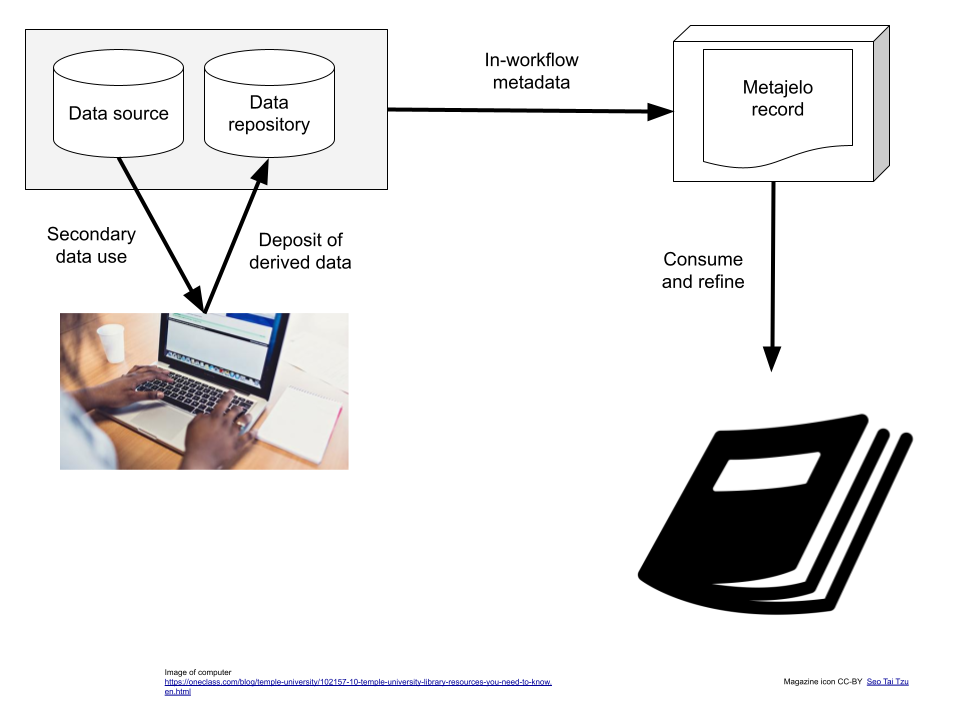
\includegraphics[width=\textwidth]{text/images/metajelo drawing.png}
    \caption{Typical secondary-use of research data}
    \label{fig:usecase}
\end{figure}

\subsection{Current Metadata Infrastructure and Use Cases}
The current metadata infrastructure should be expected to work well for open-access data deposits. Deposits are encouraged in known repositories such as \ac{ICPSR}, Zenodo, or the \urlcite{https://osf.io}{Open Science Framework}, which have been vetted according to certain criteria by the journals themselves.

But what if an author has deposited the information in a reputable but unlisted repository, for instance the \urlcite{https://ada.edu.au/}{Australian Data Archive}? Emails are to be exchanged, and some case-by-case vetting of repositories, their reliability, and whether they assign \ac{DOI} is performed. FAIRsharing.org and re3data are invoked to ascertain their policies. 

In the Appendix, we demonstrate for three cases that this infrastructure - DataCite, re3data, and FAIRsharing - will fail on even simple scenarios. In all cases, we attempt to ascertain \textit{existence}, \textit{access rules} (terms of use and licenses), and \textit{persistence} (preservation policies) via machine-readable metadata. We fail to collect complete information in  all cases. Furthermore, as of the writing of this article, and presumably for some time yet, this infrastructure simply cannot support scenarios that use broadly available restricted-access data. By ``broadly available restricted-access'', we mean that a non-trivial fraction of a research community can be granted access to these data, which are restricted-access only for reasons of confidentiality. This scenario is quite common - it applies to clinical data in psychology as much as demographic data collected by national statistical agencies in every country in the world. 

The three cases are as follows. First, we show that a user-initiated data deposit of a digital  object at  \urlcite{https://www.openicpsr.org}{openICPSR}, properly recorded in DataCite, can at best reveal \textit{existence}, but cannot reveal the remaining attributes (\textit{access rules} and \textit{persistence}) through queries to the infrastructure. A customized parser can ascertain the \textit{license} by querying the landing page of the object. Queries to DataCite fail to elicit the  license because it is optional. Queries to re3data fail because a record cannot be found using information available through the \ac{DOI}, in particular, the name of the repository. Cheating somewhat, when we force a query to re3data's entry for \ac{ICPSR} \parencite{Re3data-icpsr}, it fails to yield correct information, presumably because the record is not maintained by ICPSR staff, and does not hold information on openICPSR policies. We fail to ascertain the preservation policy through queries to all sources, and only subject-matter expertise can find the information on ICPSR's website. 

The second query is for the \ac{PSID} Geospatial Data \parencite{psid-geodata}. The \ac{PSID} is a longitudinal household survey conducted by the University of Michigan, which began in 1968. More than 4000 peer-reviewed publications have used the data \parencite{psid-homepage}. The data are available without cost to researchers - but they do require that terms of use be agreed to before downloading, through registration. This is accurately reflected in the r3data entry for the \ac{PSID} \parencite{Re3data-psid}. However, we are considering the Geospatial Data, which is restricted data. re3data fails to record any information for this access mechanism. Furthermore, although \ac{PSID} has acted as a data curator for its own data for 50 years, it does not assign a \ac{PID} to the data. DataCite has no information on any  \ac{PSID} data holdings, which are only available through the \ac{PSID} website. Until recently, both non-restricted and restricted data could not be deposited at journal websites or other repositories, as per the terms of use.\footnote{This has changed recently with the introduction of an openICPSR-hosted \ac{PSID} repository, but see the issues above.} Finally, although the \ac{PSID} has, of course, a 50-year track record, no statement can be found on the website attesting for preservation plans, or for versioning of data (preservation of prior versions).\footnote{Personal communication in November 2018 with David S. Johnson, at the time Director of the \ac{PSID}, indicates that all versions of non-restricted and restricted data are preserved in a dark archive.}

The third example is a confidential dataset made available by a \ac{NSO}, in this case the U.S. Census Bureau, although it is typical of microdata holdings by \ac{NSO} around the world. The \ac{LBD} \parencite{LBD,MirandaJarmin2002} is one of the most widely used microdata files in the \ac{FSRDC} system. The \ac{FSRDC} system is used by nearly 700 researchers at 29 locations around the United States \parencite{u.s._census_bureau_center_2018}. As with the \ac{PSID}, entries for the U.S. Census Bureau exist on re3data \parencite{Re3data-uscb}, but have no information on the \ac{FSRDC}. No \ac{PID} have yet been assigned to any datasets. Furthermore, no data can be removed from the \ac{FSRDC}. Researchers must thus rely on the U.S. Census Bureau for preservation. In addition to the \ac{LBD} itself, which is presumably covered by a record schedule, detailing its preservation period, researchers also need to consider the preservation of any derivative files they wish to make available as part of their research. If these are aggregated results (model coefficients, etc.), they are released by the U.S. Census Bureau to the researcher. Microdata cannot be released. Most of this information is provided to researchers when they obtain access, but cannot easily be communicated to journal editors or readers of articles. Nevertheless, as we have argued  
\iftoggle{blind}{[BLINDED]}{\parencite{Lagoze2017-qv}} and experienced in our own research 
\iftoggle{blind}{[BLINDED]}{\parencite{AbowdVilhuber2005,AbowdEtAl2009c,McKinneyEtAl:submitted:2017}}, it is definitely feasible to do reproducible research in this environment. The difficulty consists in communicating that information, in a reliable fashion, to editors, referees, and readers.




\subsection{Common Denominator}
We have chosen three types of datasets -- public-use, restricted-access with light restrictions, restricted-access with strong restrictions --, curated by three different institutions -- an open repository, a panel survey  provided by a recognized leader in the field, and confidential business microdata provided by one of the largest and oldest \ac{NSO} in the world -- all with impeccable data curation reputations. The choice is idiosyncratic, but it presumably is symptomatic of the still young state of the metadata infrastructure. We don't believe these examples are exceptions - similar institutions exist all over the world, and we could as easily have done such examples with data from Australia \parencite{PTKLYP_2018}, Germany (Research Data Centre (FDZ) of the German Federal Employment Agency (BA) at the Institute for Employment Research (IAB)). Presumably, counterexamples can be given. But journal editors and authors need such mechanisms to be broadly feasible if they are to use them. At present, that is not the case.

We set out to accomplish this by designing a  metadata package, drawing on existing schema used within the infrastructure, but populating it in a decentralized fashion, at the point of first use: the journal submission system, or if the researcher uses a reproducible workflow, at data acquisition by the researcher. An associated application can leverage the metadata infrastructure where it does provide information,  and pre-fill any fields. However, when ambiguous responses are obtained, or no information is available, the researcher can provide guided or verbatim answers. At both points in time, the researcher has the best incentives to provide the information accurately -- the acceptance of the submission may depend on the accuracy of the information -- and the most timely recollection of where to obtain the information.

